\documentclass[conference]{IEEEtran}

\usepackage[utf8]{inputenc}
\usepackage{amsmath,amsfonts,amssymb,bm}
\usepackage{graphicx}
\usepackage{booktabs}
\usepackage{multirow}
\usepackage{array}
\usepackage{cite}
\usepackage{xcolor}
\usepackage{tikz}
\usetikzlibrary{arrows.meta,positioning,calc}
\usepackage[hidelinks]{hyperref}

\newcommand{\method}{AudioMimic}
\newcommand{\cof}{Commit Forcing}
\newif\ifshowpapertodos
% Keep evidence gaps visible in the collaborative draft; disable only after review.
\showpapertodostrue
\newcommand{\papertodo}[1]{%
\ifshowpapertodos
\par\smallskip\noindent
{\color{red!75!black}\textbf{TODO:} #1}
\smallskip\par
\fi}

% Research draft updated 2026-09-08; see REVISION_NOTES_20260908.md.
\title{AudioMimic: Causal Humanoid Dance Generation and Execution}

% \author{\IEEEauthorblockN{Tianhu Peng et al.}
% \IEEEauthorblockA{UCL Robotics Institute, University College London}}

\begin{document}
\maketitle

\begin{abstract}
Humanoid dance should be coherent and expressive, appropriate to the music being heard, and realizable by a physical controller. We present \method{}, a robot-native causal dance generation and execution system. Its kinematics-guided discrete--continuous (D+C) representation assigns complementary coarse-structure and fine-detail roles through explicit supervision and jointly decodes both into native robot motion. \cof{} constructs sampled reference transitions and trains continuation from their committed history and reconstructed boundary states. A frozen causal music model supplies timestamped forecasts from arrived audio, and a reference bridge connects committed motion to a fixed SONIC whole-body tracker. Evaluation separates music--motion matching, explicit rhythmic and dynamic adaptation, and dance quality at generation and execution layers. Formal generator comparisons and controlled replay characterize musical matching and downstream tracking limitations. In a two-training-seed codec study, adding the continuous branch reduces structure/detail reconstruction error by approximately 30\%/45\% relative to discrete-only decoding. The proposed supervision raises the discrete-to-continuous structural intervention ratio from 1.20 to 1.41, while continuous-code effective rank reaches 15.1 of 16, supporting a measurable complementary representation.
\end{abstract}

\papertodo{Working draft, not submission-ready. Open evidence gates are indexed
as T01--T12 in TODO.md. Existing pilot results must not be promoted to general
performance, hardware, or safety claims before the corresponding gates close.}

% ================================================================
\section{Introduction}
% ================================================================
Music-to-dance systems have established strong offline choreography and, increasingly, streaming generation~\cite{tseng2023edge,ji2026discoforcing}. A live humanoid must additionally reconcile three requirements: only arrived audio is observable, reference blocks must be committed before action deadlines, and physical execution should retain the intended dance. A convincing animation, a real-time generator, and a stable robot are therefore distinct achievements. None alone establishes music-adaptive physical performance.

Our objective is not simply to make a robot move when music starts. Different music should elicit \emph{appropriately different} dance: changes in rhythm, accents, and musical character should be reflected without sacrificing coherent movement. Conversely, changing a soundtrack should not earn credit merely because the generated trajectory changes. This motivates evaluating cross-modal matching, explicit musical response, and motion quality separately, then asking whether those properties survive execution.

A robot-native representation must capture both whole-body organization and expressive local dynamics under the same causal boundary state. A discrete vocabulary alone can constrain fine variation, whereas an undifferentiated continuous latent does not explicitly assign structural responsibility. Our kinematics-guided D+C design makes this division testable: a discrete branch learns designated coarse kinematic structure, a continuous branch supplies complementary detail, and both are decoded and committed together. The contribution is this robot-native, supervised division of labor and its coupling to streaming generation, not the invention of combining discrete and continuous latents.

Teacher Forcing does not expose the planner to this deployment history. Training receives the target motion and target boundary state, while streaming inference receives sampled structure, generated detail, decoded robot motion, and a state reconstructed from that motion. Generated-history objectives reduce this mismatch~\cite{bengio2015scheduled,lamb2016professor,chen2024diffusionforcing}, but a robot planner must close all parts of the transition together. A method that changes only the token history, or preserves a teacher-provided component inside the generated transition, can still train on a context that cannot occur in the same form after deployment commitment.

We address the generated-history mismatch with \cof{}. A first pass samples structure and detail, commits them as one reference block, decodes native G1 motion, and reconstructs its boundary state. A second pass learns continuation from that generated history--state pair. This closure concerns the reference process: the reconstructed state is not a measurement of physical execution. SONIC supplies the downstream state-feedback controller~\cite{luo2026sonic}.

The music interface rolls a frozen forecaster forward from an observed prefix without future-waveform access. However, a nominal forecast horizon is not the horizon available to an action: audio processing, forecasting, publication cadence, and planning consume its lead. Furthermore, even an on-time reference can lose dynamics during tracking. We consequently evaluate condition content, condition age, and execution separately instead of attributing every offline--online difference to one model. These diagnostics support the musical-dance objective; they do not replace evidence of musical suitability or aesthetics.

At every cycle, the system predicts 0.53~s of motion, commits 0.27~s, updates its reference-derived state, and replans. Figure~\ref{fig:architecture} shows the generation loop; downstream execution is evaluated through separately recorded target and measured states. Startup is another distributional boundary: a private generated prefix, an interpolated dance pose, and a publicly generated standing transition are not interchangeable initial conditions.

This research draft organizes the work around three contributions, with evidence and remaining controls reported separately:
\begin{itemize}
    \item \textbf{Kinematics-guided D+C motion representation and generation:} explicit coarse-structure and complementary-detail supervision for native robot motion, with branch interventions that test the intended division of labor;
    \item \textbf{Commit Forcing:} training on atomically sampled and committed structure/detail references and their reconstructed boundary states, aligning the continuation context with deployment; and
    \item \textbf{Causal music-to-robot execution:} timestamped predicted-music conditioning and a reference interface to fixed SONIC control, evaluated through MMR, music adaptation, and dance quality at generation and execution layers.
\end{itemize}

\papertodo{T02--T04: close matched learning and music controls before claiming
Commit-Forcing gains, complete D+C superiority, or an injection-architecture winner.}

% ================================================================
\section{Related Work}
% ================================================================
\subsection{Music-Conditioned Dance Generation}
FACT on AIST++~\cite{li2021aist} established large-scale music-conditioned 3D dance generation, and Bailando~\cite{siyao2022bailando} introduced discrete choreographic memory with an autoregressive dance prior. EDGE~\cite{tseng2023edge} uses Jukebox features~\cite{dhariwal2020jukebox} and Transformer diffusion for editable long-form dance, while FineDance~\cite{li2023finedance} provides fine-grained full-body choreography data. LODGE~\cite{li2024lodge} organizes long dance through coarse-to-fine primitives; MEGADance~\cite{yang2025megadance} and OpenDance~\cite{zhang2026opendance} extend genre control and multimodal choreography. These systems establish strong offline generation and data foundations. Our target is the complementary deployment problem in which a native robot-motion prefix is committed before the next causal plan is produced.

\subsection{Learning from Generated History}
Scheduled Sampling~\cite{bengio2015scheduled}, Professor Forcing~\cite{lamb2016professor}, and Diffusion Forcing~\cite{chen2024diffusionforcing} address the mismatch between teacher-provided training histories and generated inference histories. MotionStreamer~\cite{xiao2025motionstreamer} introduces Two-Forward, which inserts teacher-conditioned first-pass predictions into the ground-truth latent trajectory to construct a hybrid second-pass context. This reduces exposure bias but does not train on a coherent trajectory produced by the deployment sampler. MotionStream~\cite{jiang2025motionstream} and DiscoForcing~\cite{ji2026discoforcing} further develop causal streaming motion generation. In contrast, \cof{} samples a complete deployment-form plan, commits and decodes it, reconstructs the resulting robot state, and learns the following plan from that generated history--state pair.

\subsection{Coarse-to-Fine Motion Decoupling and Humanoid Generation}
VQ-VAE~\cite{vandenOord2017vqvae} provides the standard learned discrete codebook. T2M-GPT~\cite{zhang2023t2mgpt} and MoMask~\cite{guo2024momask} use quantized motion tokens, whereas MLD~\cite{chen2023mld} models motion in a continuous latent space. DisCoRD~\cite{cho2025discord} connects discrete tokens to continuous flow decoding. Most closely, DC-Motion~\cite{wang2026dcmotion} separates human-motion structure from detail through discrete and continuous components. We decouple the two roles at both representation and training levels for robot motion: forward-kinematics supervision gives the discrete code responsibility for coarse structure, a conditional continuous generator learns finer detail, and intervention tests measure whether the separation is meaningful. The two outputs remain jointly decodable and determine the boundary state used by the next causal plan.

Physics-guided motion generation and humanoid tracking connect kinematic references to executable behavior. PhysDiff~\cite{yuan2023physdiff} injects physical projection into motion diffusion; PHC~\cite{luo2023phc}, ExBody2~\cite{ji2024exbody2}, KungfuBot~\cite{xie2026kungfubot}, BeyondMimic~\cite{liao2025beyondmimic}, and SONIC~\cite{luo2026sonic} develop scalable whole-body tracking and control. RoboPerform~\cite{li2026roboperform} directly maps audio to humanoid locomotion. \method{} instead generates persistent robot-native references under a strict causal commit contract, leaving low-level tracking to the execution layer.

\subsection{Anticipatory Music Representation}
Live Music Models~\cite{gdmlyria2025live} introduce a causal architecture for continuous music generation. Magenta RealTime~2~\cite{magenta2026mrt2} combines the SpectroStream codec~\cite{li2025spectrostream} with a frame-autoregressive music model. \method{} repurposes this model as a forecaster rather than an audio renderer: the arrived audio prefix seeds a short autoregressive rollout whose native-time hidden states represent a likely future. This creates anticipatory motion conditioning without access to future waveform samples.

\papertodo{T12: verify bibliography metadata and technical comparisons against
primary sources, especially generated-history methods and the original joint
project contributions. Do not claim first online humanoid dance.}

% ================================================================
\section{Problem Formulation}
% ================================================================
Let $\hat{x}_{<t}$ be the G1 motion already committed at time $t$, $b_t$ the boundary state derived from the final committed frames, and $m_t^{\mathrm{pred}}=\{(h_{t,j}^{\mathrm{pred}},\tau_{t,j})\}_{j=1}^{14}$ the native-time future-state sequence rolled out by the causal music model using only arrived audio. The generator samples a future reference horizon
\begin{equation}
    \hat{x}_{t:t+H-1} \sim p_\theta\!\left(
    x_{t:t+H-1}\mid \hat{x}_{<t},b_t,
    m_t^{\mathrm{pred}}\right).
    \label{eq:causal_objective}
\end{equation}
Only the first $C<H$ latent steps are committed. The unused suffix is discarded, the committed prefix updates the latent history and boundary state, and Eq.~\eqref{eq:causal_objective} is evaluated again.

The streaming contract is expressed in reader-facing time units:
\begin{itemize}
    \item 4.27~s of recently committed motion history;
    \item a 0.53-s future plan containing 16 G1 frames;
    \item commitment of the first 0.27~s, or eight frames, before replanning; and
    \item zero future-motion or future-waveform lookahead in deployable routes.
\end{itemize}

Let $\tau_k$ be the latest audio time incorporated in forecast $k$, $d_t$ the deadline for the next reference block, and $\Delta_m=1/25$~s the music-state period. The condition age and effective lead of forecast frame $j$ are
\begin{align}
    a_{t,k} &= d_t-\tau_k,\\
    \ell_{t,k,j} &= j\Delta_m-a_{t,k},\qquad j=1,\ldots,14.
    \label{eq:effective_lead}
\end{align}
The mask retains frames with positive lead under the implemented timestamp convention. Audio cutoff, publication time, fetch time, and motion deadline are recorded separately. A fresh message can therefore contain substantially fewer than 14 still-future states. The musical H14 horizon must not be confused with the eight-token motion planning horizon.

\begin{figure*}[t]
    \centering
    % Code-native diagram: reference and physical feedback are separate loops.
\resizebox{\textwidth}{!}{%
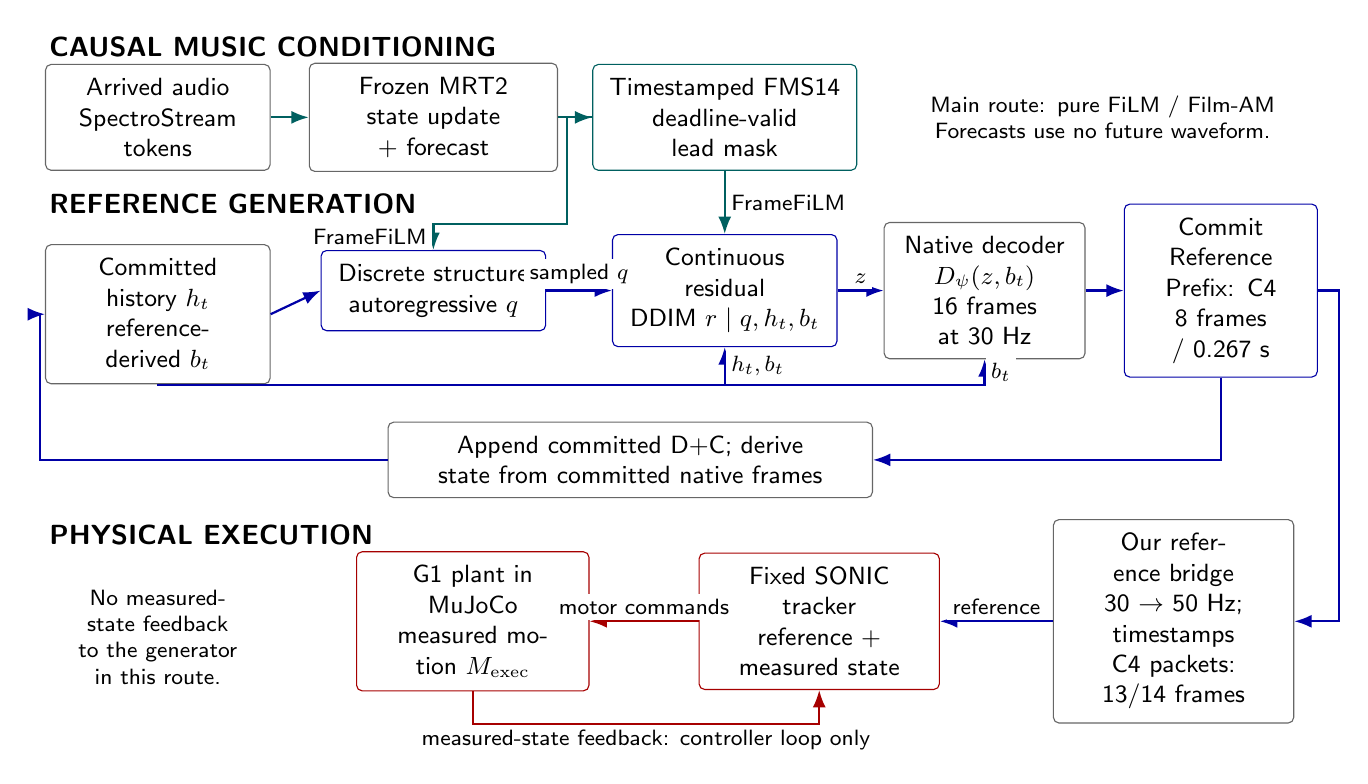
\begin{tikzpicture}[
 x=1cm,y=1cm,font=\sffamily\small,
 box/.style={draw=black!60,fill=white,rounded corners=2pt,align=center,
             text width=2.5cm,minimum height=0.95cm,inner sep=5pt},
 flow/.style={-{Latex[length=2.2mm]},thick},
 music/.style={flow,draw=teal!75!black},
 ref/.style={flow,draw=blue!65!black},
 physical/.style={flow,draw=red!65!black},
 note/.style={align=center,font=\sffamily\footnotesize,fill=white,inner sep=2pt}]
\node[anchor=west,font=\sffamily\bfseries] at (0,8.2) {CAUSAL MUSIC CONDITIONING};
\node[box] (audio) at (1.5,7.3) {Arrived audio\\SpectroStream tokens};
\node[box,text width=2.8cm] (mrt) at (5,7.3) {Frozen MRT2\\state update + forecast};
\node[box,text width=3cm,draw=teal!75!black] (mask) at (8.7,7.3)
 {Timestamped FMS14\\deadline-valid lead mask};
\node[note,text width=4.4cm] at (13.5,7.3)
 {Main route: pure FiLM / Film-AM\\Forecasts use no future waveform.};
\draw[music] (audio) -- (mrt);
\draw[music] (mrt) -- (mask);
\node[anchor=west,font=\sffamily\bfseries] at (0,6.2) {REFERENCE GENERATION};
\node[box,text width=2.5cm] (context) at (1.5,4.8)
 {Committed history $h_t$\\reference-derived $b_t$};
\node[box,draw=blue!65!black] (d) at (5,5.1)
 {Discrete structure\\autoregressive $q$};
\node[box,draw=blue!65!black] (c) at (8.7,5.1)
 {Continuous residual\\DDIM $r\mid q,h_t,b_t$};
\node[box,text width=2.2cm] (decode) at (12,5.1)
 {Native decoder\\$D_\psi(z,b_t)$\\16 frames at 30 Hz};
\node[box,text width=2.1cm,draw=blue!65!black] (commit) at (15,5.1)
 {Commit Reference\\Prefix: C4\\8 frames / 0.267 s};
\draw[ref] (context.east) -- (d.west);
\draw[ref] (d) -- node[note,above] {sampled $q$} (c);
\draw[ref] (c) -- node[note,above] {$z$} (decode);
\draw[ref] (decode) -- (commit);
\draw[music] (mask.west) -- (6.7,7.3) -- (6.7,5.95) -- (5,5.95)
 -- node[note,left] {FrameFiLM} (d.north);
\draw[music] (mask.south) -- node[note,right] {FrameFiLM} (c.north);
\draw[ref] (context.south) -- (1.5,3.9) -- (8.7,3.9)
 -- node[note,right] {$h_t,b_t$} (c.south);
\draw[ref] (8.7,3.9) -- (12,3.9) -- node[note,right] {$b_t$} (decode.south);
\node[box,text width=5.8cm,minimum height=0.7cm] (update) at (7.5,2.95)
 {Append committed D+C; derive state from committed native frames};
\draw[ref] (commit.south) -- (15,2.95) -- (update.east);
\draw[ref] (update.west) -- (0,2.95) -- (0,4.8) -- (context.west);
\node[anchor=west,font=\sffamily\bfseries] at (0,2) {PHYSICAL EXECUTION};
\node[box,text width=2.7cm] (bridge) at (14.4,0.9)
 {Our reference bridge\\30 $\rightarrow$ 50 Hz; timestamps\\C4 packets: 13/14 frames};
\node[box,text width=2.7cm,draw=red!65!black] (sonic) at (9.9,0.9)
 {Fixed SONIC tracker\\reference + measured state};
\node[box,text width=2.6cm,draw=red!65!black] (plant) at (5.5,0.9)
 {G1 plant in MuJoCo\\measured motion $M_{\rm exec}$};
\node[note,text width=2.6cm] at (1.5,0.7)
 {No measured-state feedback\\to the generator\\in this route.};
\draw[ref] (commit.east) -- (16.5,5.1) -- (16.5,0.9) -- (bridge.east);
\draw[ref] (bridge) -- node[note,above] {reference} (sonic);
\draw[physical] (sonic) -- node[note,above] {motor commands} (plant);
\draw[physical] (plant.south) -- (5.5,-0.4) --
 node[note,below] {measured-state feedback: controller loop only} (9.9,-0.4)
 -- (sonic.south);
\end{tikzpicture}%
}

    \caption{\textbf{Causal generation and fixed-controller execution.} The main pure-FiLM route supplies deadline-valid FMS14 to both branches; the residual generator also conditions on sampled discrete structure. Committed references update the generator's reference-derived history and boundary state. A separate bridge sends references to SONIC, whose physical feedback loop uses measured G1 state. No measured-state arrow feeds the generator in the reported route. LCA and RMS/FMS variants are separate controls.}
    \label{fig:architecture}
\end{figure*}

% ================================================================
\section{Kinematics-Guided Coarse-to-Fine Motion Decoupling}
% ================================================================
We decouple motion into coarse structure and finer detail at two levels. The representation assigns these roles to discrete and continuous codes. Training reinforces the same separation through kinematics-guided objectives and different structure/detail generators. The robot boundary state anchors both outputs to the pose from which execution continues.

The two branches are complementary, not two independently playable motions.
Their shared decoder allows detail to depend on sampled structure while retaining
one consistent native trajectory for commitment. Forward-kinematics supervision
connects latent roles to robot geometry rather than assuming that quantization
alone produces meaningful structure. We test reconstruction, branch intervention,
and continuous-code non-collapse separately; none implies that a discrete token
is a human-labelled dance genre or that reconstruction alone proves better dance.
\subsection{Native Motion and Boundary State}
The decoder predicts a 34-D G1 motion vector at 30~Hz,
\begin{equation}
    x_t = [\Delta p^{\mathrm{local}}_{xy},\; h,\;
    \sin \Delta\psi,\;\cos \Delta\psi,\;q^{1:29}],
    \label{eq:g1_motion}
\end{equation}
where $\Delta p^{\mathrm{local}}_{xy}$ is heading-local planar displacement, $h$ is root height, $\Delta\psi$ is yaw change, and $q^{1:29}$ are G1 joint angles. Global planar position and absolute yaw are reconstructed by a deterministic $\mathrm{SE}(2)$ accumulator.

The compact robot boundary state is
\begin{equation}
    b_t=[h,\;v^{\mathrm{local}}_{xy},\;v_z,\;\dot{\psi},\;
    q^{1:29},\;\dot{q}^{1:29}].
    \label{eq:boundary_state}
\end{equation}
It contains the pose and first-order motion required to continue the sequence. Planar and yaw acceleration remain evaluation signals rather than network inputs. The state is recomputed from the committed motion and detached before the next planning cycle.

\subsection{Representation-Level Decoupling}
The encoder maps a 16-frame segment and its boundary state to an eight-step 16-D latent. Each step is decomposed as
\begin{equation}
    z_t=e(q_t)+r_t,
    \qquad q_t\in\{1,\ldots,512\},\quad r_t\in\mathbb{R}^{16},
    \label{eq:dc_latent}
\end{equation}
where $e(q_t)$ is the discrete structure code and $r_t$ is the continuous detail code. We refer to them as the discrete (D) and continuous (C) branches. A state-conditioned decoder $D_\psi(z_t,b_t)$ reconstructs two native G1 frames. The two branches form one latent and share the same decoding and commitment horizon.

\subsection{Training-Level Decoupling}
The representation split is reinforced during training rather than inferred afterward. We construct deterministic forward-kinematics views of the predicted native motion. The full view $\Phi_f$ contains normalized native motion, boundary-aware velocities, current-root-relative positions of all 29 non-root links and two sole points, and their velocities. The coarse-structure view $\Phi_s\subset\Phi_f$ retains root, leg, and waist channels together with torso, wrist, and sole geometry. It gives the discrete branch responsibility for support, root movement, coarse pose, and endpoint organization, while the continuous branch preserves the remaining fine articulation and variation.

For encoder output $z$, quantized embedding $e$, and residual $r=z-\mathrm{sg}(e)$, the training reconstructions are
\begin{align}
    x_{\mathrm{full}} &=D_\psi(\mathrm{sg}(e)+r,b),\\
    x_{q} &=D_\psi(z+\mathrm{sg}(e-z),b),\\
    x_{\mathrm{robust}} &=D_\psi(\mathrm{sg}(e)+\mathcal{C}(r),b),
\end{align}
where $\mathrm{sg}$ stops gradients and $\mathcal{C}$ either removes the residual or adds small channel-scaled noise. The objective is
\begin{equation}
    \mathcal{L}=\mathcal{L}_{\mathrm{full}}+
    \mathcal{L}_{q\text{-}\mathrm{structure}}+
    0.25\mathcal{L}_{\mathrm{res\text{-}robust}}+
    \mathcal{L}_{\mathrm{VQ}}.
    \label{eq:codec_loss}
\end{equation}
Here $\mathcal{L}_{\mathrm{full}}$ is the mean squared error between the normalized blocks of $\Phi_f(x_{\mathrm{full}})$ and $\Phi_f(x)$. Both $\mathcal{L}_{q\text{-}\mathrm{structure}}$ and $\mathcal{L}_{\mathrm{res\text{-}robust}}$ compare the corresponding normalized blocks of $\Phi_s$ with the target structural view. Finally, $\mathcal{L}_{\mathrm{VQ}}$ is the codebook loss plus a 0.25-weighted commitment loss. Averaging each normalized block before combining them prevents high-dimensional geometry from dominating the native-motion terms.

The downstream planner retains separate structure and residual objectives. A causal classifier learns the discrete structure code with cross-entropy, while a conditional diffusion model learns the continuous code given the selected structure. Structure is sampled first; the two outputs are reunited before decoding and are committed as one motion block. Codec-level role separation is not assumed to transfer unchanged to planner samples: residual rebasing can also compensate for structural-token errors, motivating the generated-branch audit below.

\subsection{Measuring Coarse--Fine Decoupling}
The representation table uses three mechanism measures, each with one proof role. Let $\bar\Phi^S_b$ and $\bar\Phi^F_b$ denote train-split-standardized block $b$ of the declared structure view and its exact detail complement, respectively. The four equally weighted blocks are native motion, native velocity, forward-kinematic positions, and forward-kinematic velocity. For $v\in\{S,F\}$, we report
\begin{equation}
    E_v=\mathbb{E}\!\left[\sqrt{\frac{1}{4}\sum_b
    \mathrm{MSE}\!\left(\bar\Phi^v_b(\hat{x}),\bar\Phi^v_b(x)\right)}\right].
    \label{eq:view_nrmse}
\end{equation}
$E_S$ is structure NRMSE and $E_F$ is detail NRMSE; lower values mean that decoded motion better preserves the corresponding frozen view.

To test role separation rather than reconstruction alone, we exchange codes between deterministic donor pairs. Let $\Delta_D$ be structure-view displacement after swapping the discrete code while retaining the continuous code, and let $\Delta_C$ be the displacement after the complementary swap. The D/C structure-effect ratio is
\begin{equation}
    R_{D/C}=\frac{\mathbb{E}[\Delta_D]}{\mathbb{E}[\Delta_C]}.
    \label{eq:structure_effect_ratio}
\end{equation}
$R_{D/C}>1$ means that the discrete branch has the larger intervention effect on the declared structure view. This ratio is not accepted alone: the D-only reconstruction gap and the continuous-code effective rank check that the result is not obtained by collapsing the detail branch. These mechanism measures do not replace the standard FID and diversity metrics used for final generated-motion quality.

% ================================================================
\section{Learning to Continue with Commit Forcing}
% ================================================================
\begin{figure*}[t]
    \centering
    % Ordinary music-conditioned CF; no state-matched target re-encoding.
\resizebox{\textwidth}{!}{%
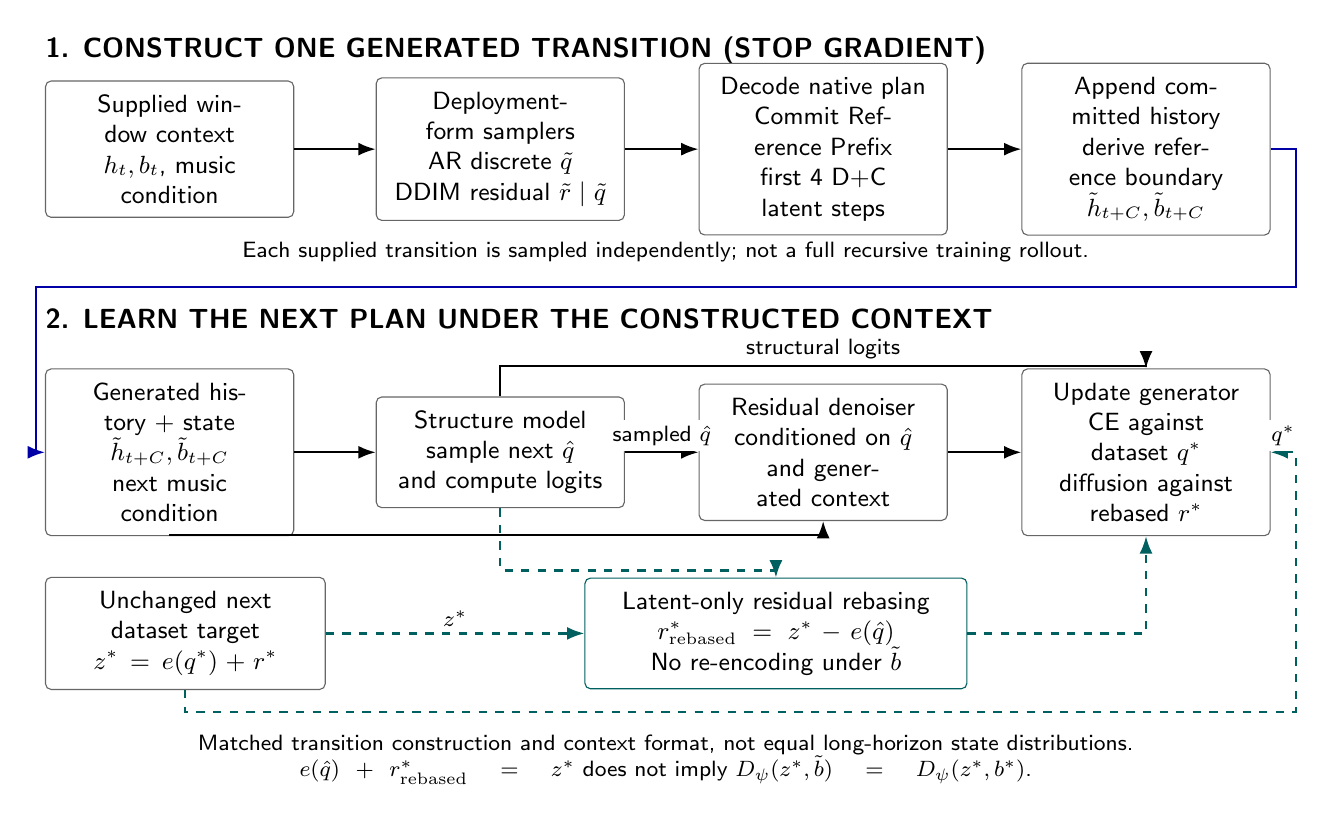
\begin{tikzpicture}[
 x=1cm,y=1cm,font=\sffamily\small,
 box/.style={draw=black!60,fill=white,rounded corners=2pt,align=center,
             text width=2.8cm,minimum height=1.05cm,inner sep=5pt},
 flow/.style={-{Latex[length=2.2mm]},thick},
 target/.style={flow,dashed,draw=teal!75!black},
 note/.style={align=center,font=\sffamily\footnotesize,fill=white,inner sep=2pt}]
\node[anchor=west,font=\sffamily\bfseries] at (0,8.05)
 {1. CONSTRUCT ONE GENERATED TRANSITION (STOP GRADIENT)};
\node[box] (start) at (1.7,6.8)
 {Supplied window context\\$h_t,b_t$, music condition};
\node[box] (sample) at (5.9,6.8)
 {Deployment-form samplers\\AR discrete $\tilde q$\\DDIM residual $\tilde r\mid\tilde q$};
\node[box] (commit) at (10,6.8)
 {Decode native plan\\Commit Reference Prefix\\first 4 D+C latent steps};
\node[box] (update) at (14.1,6.8)
 {Append committed history\\derive reference boundary\\$\tilde h_{t+C},\tilde b_{t+C}$};
\draw[flow] (start) -- (sample);
\draw[flow] (sample) -- (commit);
\draw[flow] (commit) -- (update);
\node[note,text width=12cm] at (8,5.5)
 {Each supplied transition is sampled independently; not a full recursive training rollout.};
\node[anchor=west,font=\sffamily\bfseries] at (0,4.65)
 {2. LEARN THE NEXT PLAN UNDER THE CONSTRUCTED CONTEXT};
\node[box] (context) at (1.7,2.95)
 {Generated history + state\\$\tilde h_{t+C},\tilde b_{t+C}$\\next music condition};
\node[box] (q) at (5.9,2.95)
 {Structure model\\sample next $\hat q$\\and compute logits};
\node[box] (res) at (10,2.95)
 {Residual denoiser\\conditioned on $\hat q$\\and generated context};
\node[box] (loss) at (14.1,2.95)
 {Update generator\\CE against dataset $q^*$\\diffusion against rebased $r^*$};
\draw[flow,draw=blue!65!black] (update.east) -- (16,6.8) -- (16,5.05)
 -- (0,5.05) -- (0,2.95) -- (context.west);
\draw[flow] (context) -- (q);
\draw[flow] (q) -- node[note,above] {sampled $\hat q$} (res);
\draw[flow] (res) -- (loss);
\draw[flow] (q.north) -- (5.9,4.05) -- node[note,above] {structural logits} (14.1,4.05) -- (loss.north);
\draw[flow] (context.south) -- (1.7,1.9) -- (10,1.9) -- (res.south);
\node[box,text width=3.2cm] (gt) at (1.9,0.65)
 {Unchanged next dataset target\\$z^*=e(q^*)+r^*$};
\node[box,text width=4.5cm,draw=teal!75!black] (rebase) at (9.4,0.65)
 {Latent-only residual rebasing\\$r^*_{\rm rebased}=z^*-e(\hat q)$\\No re-encoding under $\tilde b$};
\draw[target] (gt) -- node[note,above] {$z^*$} (rebase);
\draw[target] (q.south) -- (5.9,1.45) -- (9.4,1.45) -- (rebase.north);
\draw[target] (rebase.east) -- (14.1,0.65) -- (loss.south);
\draw[target] (gt.south) -- (1.9,-0.35) -- (16,-0.35) -- (16,2.95)
 -- node[note,above] {$q^*$} (loss.east);
\node[note,text width=14cm] at (8,-0.95)
 {Matched transition construction and context format, not equal long-horizon state distributions.\\
 $e(\hat q)+r^*_{\rm rebased}=z^*$ does not imply
 $D_\psi(z^*,\tilde b)=D_\psi(z^*,b^*)$.};
\end{tikzpicture}%
}

    \caption{\textbf{Commit Forcing matches the construction of a reference transition.} A stop-gradient pass samples structure and residual, commits them jointly, and derives the next reference state. The second pass uses this context while retaining the next dataset target latent. Residual rebasing preserves that latent, not decoded motion across different boundary states. Batched one-transition replacement does not imply equality with the long-horizon deployment-state distribution.}
    \label{fig:commit_forcing}
\end{figure*}

\subsection{Coarse-to-Fine Planner}
A causal Transformer autoregressively predicts eight future discrete structure codes. Conditioned on the sampled coarse structure, committed history, and boundary state, a continuous diffusion branch predicts the corresponding fine-detail codes. The two branches retain their separate classification and diffusion objectives during planner training. The detail model uses $x_0$ prediction and DDIM sampling~\cite{song2021ddim} with ten function evaluations. Decoding their sum produces a 0.53-s plan of 16 G1 frames.

\subsection{Receding-Horizon Commit}
At cycle $t$, the eight-step latent plan is
\begin{equation}
    P_t=\{(q_{t+i},r_{t+i})\}_{i=0}^{7}.
\end{equation}
The system commits the first four latent steps as references,
\begin{equation}
    P_t^{\mathrm{commit}}=\{(q_{t+i},r_{t+i})\}_{i=0}^{3},
    \label{eq:commit_prefix}
\end{equation}
decodes the eight committed motion frames, updates the recent history, and constructs the next boundary state using Eq.~\eqref{eq:boundary_state}. Both branches advance together, making the reference-state transition used for replanning explicit without assuming that generated samples retain the codec's measured division of labor.

\subsection{Commit Forcing}
\cof{} aligns training with this generated-history transition through three coupled closures, as shown in Fig.~\ref{fig:commit_forcing}.

\textbf{Sampler closure.} A stop-gradient first pass generates $\tilde{P}_t$ with the autoregressive structural sampler and multi-step residual sampler used at deployment, rather than replacing a commit with teacher-conditioned point predictions. The audited ordinary CF implementation samples each training-window transition independently from its supplied context, generally a dataset history and state. It does not recursively unroll all batch transitions into one generated trajectory. Prefix-aware training can change these starting contexts without changing this distinction. The structural plan supplied to the second prediction is sampled autoregressively from the constructed generated context.

\textbf{Commit closure.} The first four structural tokens and their residuals form one indivisible C4 commit. During the curriculum, a transition uses either the complete generated commit or the complete target commit; structure, detail, and the corresponding state are never mixed within that transition. The generated-commit probability rises to one, and the selected final method retains no target-history floor.

\textbf{State closure.} The committed latent block is decoded into eight native G1 reference frames. Those frames update the recent motion history and reconstruct the next boundary state using the same causal update as inference:
\begin{equation}
    (\tilde{h}_{t+C},\tilde{b}_{t+C})
    =\mathcal{U}(h_t,b_t,\tilde{P}_t^{\mathrm{commit}}).
    \label{eq:generated_context}
\end{equation}
A second pass learns the following horizon from this generated history--state pair. Let $z_i^*=e(q_i^*)+r_i^*$ be the target full latent and $\tilde q_i$ the structural token sampled for that prediction. The rebased residual target is
\begin{equation}
    \tilde r_i^*=z_i^*-e(\tilde q_i),
    \qquad e(\tilde q_i)+\tilde r_i^*=z_i^*.
    \label{eq:residual_rebasing}
\end{equation}
This identity preserves only the \emph{complete target latent}. The audited
music-conditioned CF path copies the next dataset $q_i^*,r_i^*$ unchanged into
the generated context and normalizes the rebased residual for diffusion
supervision. It does not re-encode the next target under $\tilde b$ or construct
a boundary-matched target trajectory. Since the decoder is state-conditioned,
\begin{equation}
 D_\psi(z_i^*,\tilde b)\ \not\equiv\ D_\psi(z_i^*,b^*).
 \label{eq:cf_state_limit}
\end{equation}
State closure ensures that the conditioning state agrees with the committed
\emph{reference}, not that the retained GT continuation is dynamically or
kinematically compatible with every generated boundary. Continuity is learned
through state conditioning and generated-context exposure, not guaranteed by
rebasing. Pose/velocity jumps and target reconstruction under both boundaries
must therefore be measured. State-matched re-encoding is a distinct objective
variant, not an implicit step of the reported CF route.

\textbf{Residual compensation.} The correction can be written as
$\tilde r_i^*=r_i^*+[e(q_i^*)-e(\tilde q_i)]$. Thus a structural error can be
absorbed by the residual target. To test whether generated D+C still exhibits
the codec's division of labor, the planned audit reports residual norm and
tails, correction-to-original-residual magnitude on labelled windows, code
mismatch rate, and discrete/residual interventions during recursive generation.
This is separate from the existing fixed-decoder codec audit. The closures
match the form and construction of one generated transition; neither target
compatibility nor long-horizon context-distribution equality follows automatically.

\papertodo{T02: run matched Teacher Forcing versus Commit Forcing and remove sampler,
commit, and state closure separately. Match parents, data, training budgets and
seeds, inference NFE, and startup. Test target compatibility under generated
boundaries and residual compensation, alongside song-level uncertainty and
long-horizon degradation.}

% ================================================================
\section{Anticipating Music without Future Audio}
% ================================================================
A causal dancer must prepare without reading future audio. Arrived audio is converted into discrete SpectroStream tokens and supplied to a frozen Magenta RealTime~2 model. We roll this prefix forward deterministically and retain 14 native 25-Hz temporal states, covering approximately 560~ms. These states are forecasts produced from arrived audio, not encodings of future waveform samples.

Each forecast state retains its native timestamp and is consumed without interpolation onto the motion grid. The deployable route uses the newest completed forecast from an earlier audio cutoff, masks states whose effective lead has expired according to Eq.~\eqref{eq:effective_lead}, and records age and valid-frame count. Cached forecasts are previously computed predictions, not oracle encodings of actual future audio. Zero-age cache replay is a latency-free diagnostic, not a deployable full-song baseline.

The main pure-FiLM route injects predicted FMS14 into both the structural and detail generators through FrameFiLM~\cite{perez2018film}; its prefix-aware variant retains that architecture. A hybrid control instead uses local cross-attention for the structural branch and FrameFiLM for detail. An RMS+FMS control combines 100 observed music-history states and 14 forecast states through FiLM-family conditioning. Here RMS denotes music states, not waveform root-mean-square amplitude. Architecture, music inputs, and startup training are separate experimental factors; FiLM-to-hybrid comparisons must account for their different parameter counts.

The service and generator run asynchronously, but their interaction is still constrained by freshness. We denote the publication target period and generator scheduling budget by S and B. S100-B140 uses a 100-ms snapshot target and starts planning with a 140-ms budget before the deadline. Reducing B can allow a newer forecast to be selected; it does not accelerate the network and reduces tolerance to compute jitter. Future-rollout timings alone exclude front-end processing, state updates, scheduling, transport, and tracking. Increasing the forecast horizon may recover lead, but also increases cost and predictive uncertainty; it is not assumed to solve this tradeoff.

\papertodo{T04/T06: complete causal past-only/static-now versus predicted-future
controls and capacity/startup-matched FiLM--LCA comparisons. Repeat content/age
interventions over songs and seeds. Audit H14 and longer horizons using effective
lead, prediction quality, and full-pipeline timing, not rollout timing alone.
An oracle substituted into a predictor-trained model is not automatically an upper bound.}

% ================================================================
\section{Startup and Physical Execution}
% ================================================================
\subsection{Matching the Public Startup Distribution}
The first publicly emitted block requires an explicit contract. A dance sequence need not begin in a two-foot standing pose. Moreover, exposing an empty-history generator differs from displaying motion after private exact-null commits. Interpolating toward an already raised foot or arm can hide the initial discontinuity in animation without establishing dynamically stable startup.

We distinguish clean startup, with no private commits or reference alignment, from a learned visible-start candidate. The latter retains the FiLM/FMS14 architecture and uses five stability-gated measured standing poses. Twenty percent of training rows are song-origin examples with empty motion history, an initial exact-null condition, and subsequent observed music prefixes; the remaining rows retain continuation training. A two-second minimum-jerk blend constructs startup targets without shifting song time, followed by codec re-encoding. Training to 6250 updates has completed, but target smoothness and codec reconstruction do not establish learned or physically executed startup success. Acceptance requires first-pose continuity, early velocity/contact and drift checks, and preservation of subsequent dance activity and musical adaptation.

\papertodo{T05: validate the u6250 startup candidate against matched old-model and
initialization controls. Evaluate untrimmed first-pose error, early velocity,
contact and forward drift, plus later activity/music fit. Compare transition
durations and initialization distributions without changing song time.}

\subsection{Fixed Tracker and Reference Interface}
We use the pretrained SONIC whole-body controller~\cite{luo2026sonic} as an external, fixed execution layer. Our bridge decodes native motion, converts the reference from 30 to 50~Hz, enforces representation and timestamp conventions, and packages reference messages. No new low-level policy or controller-training contribution is claimed. In the reported diagnostic runs, reference clipping, startup ramps, and alignment holds are disabled; timing and state watchdogs remain distinct from reference smoothing.

One C4 commit contains eight 30-Hz frames and becomes a sequence of 13 or 14
50-Hz reference frames under a continuous time grid. These messages supply motion
references, not motor torques; SONIC combines the consumed reference with measured
robot state to produce low-level control. Packet timing and future-reference
access are part of the execution protocol. The bridge and recording tools are
our integration layer, while the reported SONIC policy remains fixed. Musical
intent is specified upstream, so target tracking error alone cannot show whether
the executed dance remains appropriate to its soundtrack.

The generator updates a reference-derived boundary state, whereas SONIC closes the physical state-feedback loop. Feeding measured execution back into the generator would require matching feedback timestamps to its future planning boundary. That mechanism is not established by merely recording feedback and is not part of the reported closed-loop generation claim.

\subsection{Recorded Layers and Reconstruction Audit}
We distinguish raw generator motion $M_{\mathrm{gen}}$, the resampled reference sent by the bridge $M_{\mathrm{sent}}$, the controller's consumed target $M_{\mathrm{target}}$, and measured execution $M_{\mathrm{exec}}$. Simulated root state and feedback arrival times are retained alongside joint data. Generation-to-adaptation, delivery-to-consumption, and target-to-execution discrepancies must not be conflated.

The feedback contract distinguishes named target/measured fields in absolute
MuJoCo joint order from raw fields with different ordering and offsets.
Reconstruction is checked against the simulator before anatomical grouping
and startup comparisons. Joint-conversion debugging history and field-level
provenance are retained in the research record, not interpreted as controller
or training improvements.

\papertodo{T01: audit named and fallback feedback fields, units, default offsets,
root/quaternion conventions, and timestamps against original records. Recheck
rendered motion against the simulator and recompute affected startup/group metrics.}

% ================================================================
\section{Experiments}
% ================================================================
We ask three questions: whether the generated dance fits its soundtrack,
whether D+C/CF improve generation under matched controls, and whether musical
expression survives controller execution. Table~\ref{tab:primary_outcomes}
front-loads the available generator outcomes and the missing matched execution
rows. Representation and timing/tracking diagnostics then explain mechanisms;
their cohorts are not pooled into the primary comparison.

\begin{table*}[t]
\centering
\caption{Primary-outcome matrix, currently partial. Generator-only correct-condition
means are transcribed from the formal 18-song, three-sampling-seed report;
they are not new online execution results. Execution rows require the same cohort
and metric protocol, not substitution of the one-song A--D tracking pilot.
Song-level intervals and human judgments remain pending for this matrix;
no model is highlighted as a statistically established winner.}
\label{tab:primary_outcomes}
\small
\setlength{\tabcolsep}{6pt}
\begin{tabular}{@{}llccccc@{}}
\toprule
Model & Layer & MMR-MS $\downarrow$ & BAS $\uparrow$ & Onset--impact $r$ & FID$_k$ $\downarrow$ & FID$_g$ $\downarrow$\\
\midrule
Old D+C, FMS-FiLM & Generated & 1.367 & 0.244 & 0.067 & 276.285 & 269.407\\
Prefix-aware D+C, FMS-FiLM & Generated & 1.357 & 0.257 & 0.072 & 319.827 & 270.164\\
D+C, RMS+FMS-FiLM & Generated & 1.323 & 0.240 & 0.072 & 293.709 & 235.578\\
\midrule
Old D+C, FMS-FiLM & Executed & -- & -- & -- & -- & --\\
Prefix-aware D+C, FMS-FiLM & Executed & -- & -- & -- & -- & --\\
D+C, RMS+FMS-FiLM & Executed & -- & -- & -- & -- & --\\
\bottomrule
\end{tabular}
\end{table*}

The available outcomes are mixed: prefix-aware FiLM has a higher mean BAS than
the old FiLM model, but a worse kinetic FID; RMS+FMS has a lower learned matching
distance without the highest BAS. Onset--impact correlations are small, and
FID estimates use only 18 matched GT trajectories against 54 generated samples.
Thus these means motivate paired music controls and perceptual inspection,
not an overall quality ranking. The available song-bootstrap BAS comparison
is reported below. Completing the executed rows, song-level intervals, and
cross-paired music-fit/blinded-quality tests is the primary result priority.

\papertodo{T02--T04/T07--T10: complete matched D-only, continuous-only and TF/CF
generation controls, then the paired generation/execution outcome matrix.
Use held-out songs and independent tracker resets; do not fill missing rows
with results from incompatible diagnostic cohorts.}


\subsection{Protocol}
We train on the canonical FineDance-to-G1 pipeline~\cite{li2023finedance} at 30~Hz. Representation comparisons use two matched training seeds and 512 deterministic held-out plans per seed. The structure view uses frozen designated native channels together with torso, wrist, and foot geometry; the detail view is its exact complement. All NRMSE values use train-split statistics and the equal-weight block definition in Eq.~\eqref{eq:view_nrmse}. Donor pairs, data order, representation width, and evaluation plans are matched.

\subsection{Coarse--Fine Decoupling Audit}
This experiment tests complementary branch roles and the effect of the
supervision design. The D-only row zeros the continuous code at decoding; it
is a component ablation, not an independently trained discrete-only model.
The two full-state D+C rows compare \emph{overlapping supervision} with the
proposed projector-based supervision. Overlapping supervision trains the
discrete reconstruction on all 34 native channels with nonzero weights,
including arm detail, whereas the proposed discrete and residual-robust losses
use only the declared structural view. The full branch retains full-view
supervision. The proposed bundle also removes the auxiliary contact head and
legacy endpoint/physical penalties; this is not a single-loss toggle.
Appendix~\ref{app:supervision} lists channels and coefficients. The compact-state
row then changes the boundary representation under the proposed supervision.

\begin{table}[t]
\centering
\caption{Representation mechanism ablation (two-seed means). NRMSE measures reconstruction fidelity in frozen structure/detail views; $R_{D/C}$ measures their intervention-based division of labor.}
\label{tab:decoupling_audit}
\scriptsize
\setlength{\tabcolsep}{2pt}
\begin{tabular}{@{}lccc@{}}
\toprule
Variant & \shortstack{Struct.\\NRMSE $\downarrow$} & \shortstack{Detail\\NRMSE $\downarrow$} & $R_{D/C}$ $\uparrow$\\
\midrule
D only ($C=0$) & 0.361 & 0.449 & --\\
D+C, overlapping supervision & 0.303 & 0.270 & 1.20\\
D+C, proposed objective & \textbf{0.250} & \textbf{0.243} & 1.41\\
Ours, compact state & 0.252 & 0.245 & \textbf{1.41}\\
\bottomrule
\end{tabular}
\end{table}

Each column answers a separate mechanism question. Structure NRMSE tests coarse-motion fidelity, detail NRMSE tests whether the continuous branch restores complementary motion, and $R_{D/C}$ tests whether the two branches exert the intended relative effects. Adding the continuous branch to the selected model reduces structure and detail NRMSE by 30\% and 45\% relative to D-only decoding. With the boundary state held fixed, replacing the legacy overlapping objective with the proposed kinematics-guided objective raises $R_{D/C}$ from 1.20 to 1.41 while reducing both reconstruction errors. The compact state preserves these gains, and both of its seed-specific paired-bootstrap 95\% confidence lower bounds for $R_{D/C}$ remain above 1.38. Its continuous code supplies 45\% complementary-detail gain with an effective rank of 15.1 out of 16. Together, the reconstruction, intervention, and non-collapse evidence support a discrete coarse-structure branch paired with a continuous detail branch.

\papertodo{T03: add recursive discrete-only, independently trained continuous-only,
and direct motion-space controls under a matched contract. Audit historical
representation-table receipts. Fixed-q0 zero-residual decoding is only a component
counterfactual; q0 genre semantics remain unproven.}

\subsection{Three-Block Outcome Protocol}
The primary outcomes are (1) frozen MMR matching, (2) rhythm and dynamic response
to the soundtrack, and (3) dance quality. We prioritize MMR-MS and matched-audio
preference, BAS and onset--impact correlation, and motion distribution/diversity
with blinded aesthetics. These are assessed on both generated references and
measured execution under matched songs, sampling seeds, duration, and audio
time. No post-hoc music shift improves a primary score. Startup is evaluated
separately rather than only trimmed away. Detailed definitions, calibration,
and status are in Appendix~\ref{app:evaluation}.

Music-change tests must demonstrate appropriate adaptation rather than merely
different trajectories: each of two generated dances is paired with both
soundtracks, with histories and random draws controlled. Correct-pair preference
must survive SONIC execution and agree with independent listening judgments.
Blinded motion-only viewing separately tests naturalness and aesthetics.
Phrase and affect endpoints are optional extensions, not prerequisites for the
core rhythm/dynamics/music-fit claim. Confidence intervals use songs as clusters;
sampling seeds are repeated measurements, not independent songs.

\subsection{Generator Cohorts and Evaluator Calibration}
The current formal generator matrix compares old DC-FILM-F, Film-AM, and
RMS100+FMS14 DC-RF-EQ on 18 FineDance songs, three sampling seeds, and seven
condition settings: correct, exact-null, same-track wrong-time, same-genre
wrong-track, cross-genre wrong-track, and shifts of $\pm4$ music frames. Sampling
seeds are repeats of a checkpoint, not independent training seeds. Hybrid and
additional routing/style experiments include smaller diagnostic cohorts and are
not ranked against this matrix without matching their protocols.

Song-cluster bootstrap gives a Film-AM minus old DC-FILM-F BAS difference of
$+0.0129$ (95\% CI $[-0.0108,0.0375]$). Film-AM also has lower motion-energy and
jerk measures. Thus Film-AM is a reproducible operational baseline, not an
established winner in either dance quality or musicality. In a separate six-song,
three-sampling-seed fixed-q0 counterfactual, restoring the predicted residual
reduces the joint-jerk measure from 1588.6 to 291.3 and wrist jerk from 1052.8 to
153.3. This supports a local-dynamics role for the residual, but is not a
recursively generated discrete-only comparison.

The FineDance-only frozen music--motion evaluator supports the current formal
comparisons. A multi-dataset calibration candidate was revised to identify AIST++
music independently of dancer/performance identity: multiple performances of one
song are valid positives, not distinct songs or false negatives. Its held-out
cohort contains 28 independent songs, including ten AIST++ and 18 FineDance songs.
Overall and FineDance calibration gates pass, but AIST++ wrong-song, same-style,
and same-tempo control confidence intervals cross zero. This candidate is not yet
accepted as a cross-dataset ranking metric. Blinded perceptual evaluation remains
pending; no current proxy score is interpreted as an aesthetic verdict.

\papertodo{T08--T10: freeze final song-level splits and metrics, account for
training versus sampling seeds, and include failed attempts. Close per-dataset
evaluator calibration gates and conduct blinded quality, musicality, and execution
retention studies before aesthetic or cross-dataset ranking claims.}

\subsection{Condition Content and Age Attribution}
We hold the Film-AM checkpoint, sampling seed 1234, motion initialization, and
selected audio cutoffs fixed. A matched archive for song 098 supplies cached and
live MRT2 conditions. Each replay begins at audio time 5.8~s with empty motion
history and generates 225 commits, or 1800 frames at 30~Hz. This is an artificial
60-s paired segment, not end-to-end song-onset generation. All conditions use
predicted FMS14 rather than actual future audio.

Table~\ref{tab:age_conditions} defines four interventions. A is the ideal-age
reference; B and C change only the injected consumption-age trace. D changes
condition content relative to C while retaining the new trace. The old trace is
from a 250-ms-budget online run; the new trace is from S100-B140. The new traced
run has age p50/p95 of approximately 273/326~ms and a median of eight valid
future frames. Its 60-s online execution completes all 225 commits with no
recorded deadline misses or holds. This is sample-level feasibility evidence,
not a success rate over all attempts.

\begin{table}[t]
\centering
\caption{Paired age-attribution conditions. Cached content is predicted music,
not ground-truth future audio.}
\label{tab:age_conditions}
\small
\begin{tabular}{@{}lll@{}}
\toprule
Group & Content & Consumption age\\
\midrule
A & Cache & Zero\\
B & Same cache & Old measured trace\\
C & Same cache & S100-B140 trace\\
D & Matched live & Same S100-B140 trace\\
\bottomrule
\end{tabular}
\end{table}

\begin{table}[t]
\centering
\caption{Generation discrepancy for the single-song paired segment. Joint RMSE
measures trajectory sensitivity, not dance quality.}
\label{tab:age_discrepancy}
\small
\begin{tabular}{@{}lcc@{}}
\toprule
Pair & Joint RMSE (rad) & Planar-root RMSE (m)\\
\midrule
A--B & 0.2281 & 0.3238\\
A--C & 0.2064 & 0.2650\\
C--D & 0.1084 & 0.2895\\
A--D & 0.2043 & 0.2467\\
\bottomrule
\end{tabular}
\end{table}

The A--C joint discrepancy is approximately 9.5\% lower than A--B
(Table~\ref{tab:age_discrepancy}). This quantifies a change in distance to the
ideal-age cached trajectory, not a 9.5\% gain in musicality or online quality.
The C--D comparison also shows residual content sensitivity. These distances are
not additive error components: autoregressive rollout and content--mask
interactions prevent assigning percentages of the total quality gap to MRT2,
age, and tracking. A complete factorial study and repeated songs/seeds remain
necessary for broader attribution.

\subsection{Fixed-Reference SONIC Execution}
We replay each A--D trajectory through the same SONIC controller as C4 packets,
with no preview, clipping, ramp, or alignment hold. References are resampled to
50~Hz at playback rate one. These experiments isolate tracking of previously
generated motion; neither cached nor live-labelled replay performs online music
inference during execution. All four records cover approximately 60~s. We trim
the first two seconds for the steady-state statistics below; startup requires
its own untrimmed analysis.

For active joint $i$, define amplitude and dynamic retention as
\begin{align}
 R_i^{\mathrm{amp}} &=\frac{P_{95}(q_i^{\mathrm{exec}})-P_5(q_i^{\mathrm{exec}})}
 {P_{95}(q_i^{\mathrm{target}})-P_5(q_i^{\mathrm{target}})},\\
 R_i^{\mathrm{dyn}} &=\frac{\mathbb{E}[(\dot q_i^{\mathrm{exec}})^2]}
 {\mathbb{E}[(\dot q_i^{\mathrm{target}})^2]}.
\end{align}
The target peak-to-peak range must exceed 0.02~rad to enter the active-joint summary;
ratios with near-zero denominators are excluded.
We report medians of joint-wise ratios. The dynamic statistic is not physical
energy in joules or a whole-body total-energy ratio. Lag is estimated over a
$\pm0.5$-s range at 50~Hz, hence on a 20-ms grid.

\begin{table}[t]
\centering
\caption{Fixed-reference tracking, excluding the first 2~s. Each row is one run.
All four estimated lags are 40~ms; this is not a universal controller latency.}
\label{tab:tracking_retention}
\small
\setlength{\tabcolsep}{4pt}
\begin{tabular}{@{}lccc@{}}
\toprule
Group & \shortstack{Aligned RMSE\\(rad)} & Median $R^{\mathrm{amp}}$ & Median $R^{\mathrm{dyn}}$\\
\midrule
A & 0.1421 & 0.869 & 0.496\\
B & 0.1281 & 0.858 & 0.428\\
C & 0.1394 & 0.877 & 0.412\\
D & 0.1431 & 0.901 & 0.411\\
\bottomrule
\end{tabular}
\end{table}

Substantial dynamic attenuation coexists with moderate amplitude retention
(Table~\ref{tab:tracking_retention}). With corrected anatomical grouping, median
arm power retention in the 3--8~Hz band ranges from approximately 0.130 to 0.142,
versus 0.363--0.542 for the legs. This motivates examining fast arm events rather
than relying only on whole-body position RMSE. Nevertheless, high-frequency
content can include jitter; restoring all spectral power is not inherently
desirable. Native/retargeted GT controls and blind paired viewing are required
to determine which attenuated components carry meaningful musical expression.

\papertodo{T07: repeat native/retargeted GT and generated-reference tracking with
independent resets; control full/C4 future-reference access and initial state.
Check event-specific and perceptual loss before proposing tracker-aware adaptation.
Median joint-wise retention is not total physical energy or an error-attribution share.}

\subsection{Remaining Controlled Evaluations}
We retain three distinct comparison axes: generated motion from matched
cache/live conditions; fixed-motion full versus C4 reference delivery; and
actual online generation with execution. Full-packet delivery can expose more
future reference than C4, so it is not merely a packet-count intervention.
Further runs must control initialization, future-reference access, timestamps,
and recording coverage. Final reliability statistics must include aborted
attempts, not only successful retries. Audio-to-action timing, forecast age,
valid-frame count, plan-time tails, misses/holds, and simulation real-time
factor accompany motion and musicality scores. These controls are necessary
before extrapolating paced-file MuJoCo results to microphone input or real G1
hardware.

% ================================================================
\section{Discussion}
% ================================================================
\textbf{What is supported.} The representation ablation supports complementary
structure/detail roles. The matched replay demonstrates sensitivity to
consumption age even when condition content is held fixed. Tracking the same
recorded trajectories reveals another loss of motion dynamics. Improving
condition timing therefore does not, by itself, establish preserved physical
expression; conversely, ideal-age cached conditions do not eliminate tracking
attenuation.

\textbf{What remains unresolved.} The age-attribution study uses one song and one
sampling seed with an artificial empty-history start. Its trajectory RMSE is
not an aesthetic score. Physical tracking results are MuJoCo measurements,
not a real-hardware validation or safety guarantee. The learned standing-start
candidate has not passed its generation/execution gates. FineDance formal
comparisons, smaller mechanism pilots, and the two-training-seed codec study
have different cohorts and cannot be pooled. Additional architecture and
Commit-Forcing ablations, a calibrated cross-dataset evaluator, and human
judgments are still needed.

\textbf{Research direction.} We prioritize startup train--deployment consistency
and deadline-effective music conditioning before adding model branches. If
tracking-aware reference adaptation is pursued, it should preserve validated
musical events under a fixed controller and be compared with simple smoothing
and clipping. The controller remains fixed in the present study. The final held-out set must be
separate from songs repeatedly used to tune the present diagnostics.

\papertodo{T11/T12: obtain real-G1 records only if hardware claims are retained;
separate edited showcases from continuous trials and report interventions. Finalize
authorship, primary-source citations, figures, venue format and page budget.
Disable visible TODOs only after each retained claim has evidence or is narrowed.}

% ================================================================
\section{Conclusion}
% ================================================================
We presented \method{} toward coherent, expressive robot dance that responds
appropriately to music as it arrives. Kinematics-guided D+C modeling assigns
complementary coarse-structure and fine-detail roles in native robot motion;
\cof{} trains continuation from jointly committed generated references and
their boundary states. Timestamped causal forecasts and a reference bridge
connect this generator to fixed SONIC execution. The evaluation separates MMR,
explicit music adaptation, and dance quality/aesthetics, with runtime and
tracking diagnostics identifying where intended behavior is lost. Existing
representation and layered studies support specific mechanisms, not a claim
that online executed dance already matches offline animation. Matched learning
ablations, learned-startup validation, and music-fit and aesthetic judgments at
both generation and execution remain necessary for that broader conclusion.

\appendices
\section{Detailed Evaluation Definitions and Coverage}
\label{app:evaluation}
\begin{table*}[!t]
\centering
\caption{Three complementary evaluation blocks. R: reported in existing formal
or diagnostic cohorts; I: implemented or exploratory, but final validation or
coverage is incomplete; P: planned. R does not mean that every model, song, and
execution layer has been evaluated. No aggregate quality score is used.}
\label{tab:evaluation_matrix}
\small
\renewcommand{\arraystretch}{1.16}
\setlength{\tabcolsep}{0pt}
\begin{tabular}{@{}>{\raggedright\arraybackslash}p{0.15\textwidth}
                    @{\hspace{0.02\textwidth}}
                    >{\raggedright\arraybackslash}p{0.36\textwidth}
                    @{\hspace{0.02\textwidth}}
                    >{\raggedright\arraybackslash}p{0.45\textwidth}@{}}
\toprule
\textbf{Block} & \textbf{Metrics and direction} & \textbf{Question and evidence status} \\
\midrule
\textbf{1. MMR} & MMR-MS, MMDist $\downarrow$; audio-to-motion and motion-to-audio R@K $\uparrow$, median/mean rank $\downarrow$ &
Does an independent learned evaluator associate the motion with its music?
\textbf{R:} FineDance matching/retrieval subsets. \textbf{I:} cross-dataset calibration;
not a direct aesthetic judgment. \\
\midrule
\textbf{2. Music adaptation} & BAS $\uparrow$; beat-event coverage and timing; onset--motion correlation and response lag &
Does the movement respond to the soundtrack's rhythm and dynamics?
\textbf{R:} BAS and beat diagnostics in formal cohorts; onset/impact diagnostics in
layer analysis. Event coverage is not a mandatory one-to-one beat assignment. \\
& Tempo/phase, section response, style/affect fit; correct versus swapped-audio preference &
\textbf{I:} tempo/style diagnostics. \textbf{P:} validated phrase/affect endpoints
and blinded cross-paired music-fit study at generation and execution. \\
\midrule
\textbf{3. Dance quality and aesthetics} & FID$_k$/FID$_g$/FID$_L$ $\downarrow$;
Div$_k$/Div$_g$/Div$_L$ and same-song multimodality $\leftrightarrow$GT &
Is the motion distribution plausible and varied? \textbf{R:} kinetic/geometric
and learned-metric subsets. Small GT cohorts limit FID interpretation. \\
& Velocity, acceleration, jerk, activity and repetition $\leftrightarrow$GT;
boundary jumps and physical violations $\downarrow$ &
\textbf{R:} motion-dynamics and continuity diagnostics. \textbf{I:} contact/skating
proxies and standardized physical checks. Low activity or low jerk alone is not success. \\
& Blinded naturalness, smoothness, expressiveness and aesthetics $\uparrow$ &
\textbf{P:} silent-video quality study and paired reference/execution study;
no perceptual superiority is claimed from existing proxy scores. \\
\bottomrule
\multicolumn{3}{@{}l@{}}{\footnotesize $\uparrow$: higher is better; $\downarrow$:
lower is better; $\leftrightarrow$GT: match the paired ground-truth distribution.} \\
\end{tabular}
\end{table*}

\subsection{Shared Evaluation Contract}
Table~\ref{tab:evaluation_matrix} separates three questions: learned cross-modal
matching (MMR), explicit music adaptation, and dance quality/aesthetics. They are
complementary, not independent quantities that can be added into one score.
The third block concerns the motion itself; the first two concern its relation
to the soundtrack. Distributional, rhythmic, physical, and perceptual evidence
follows established dance evaluation practice~\cite{li2021aist,tseng2023edge,li2024lodge,ji2026discoforcing,li2026roboperform}.

The calibration chain comprises paired human motion ($O_{\mathrm{Human}}$), its
GMR-retargeted G1 counterpart ($O_{\mathrm{G1}}$), and execution of that G1 target
($O_{\mathrm{Exec}}$). Generated motion is evaluated through the recorded
$M_{\mathrm{gen}}$--$M_{\mathrm{sent}}$--$M_{\mathrm{target}}$--$M_{\mathrm{exec}}$
chain. The generator is trained directly in the G1 domain; online output is not
retargeted again. The final protocol applies all three blocks to both
$M_{\mathrm{gen}}$ and $M_{\mathrm{exec}}$ where the evaluator's domain calibration
permits it. Existing tracking recordings do not imply that this complete scoring
matrix has already been computed.

Audio time, crop duration, rig, feature normalization, evaluator checkpoint, and
aggregation rules are fixed within a comparison. Music scores use the recorded
audio--action clock, without independently shifting each video to improve fit.
Lag-compensated tracking is a separate diagnostic. Startup is reported untrimmed
and separately from the post-startup interval. Missing inputs, unsupported
domains, and unvalidated endpoints are marked N/A, not treated as zero-quality
samples or silently removed. Music-conditioning features are not evaluation
metrics; the learned evaluator is frozen independently of generator fitting.

The source song, rather than the frame, is the statistical unit. Sampling seeds
are repeated measurements within a song, distinct from training seeds and
tracker resets. Final comparisons require a held-out manifest, all eligible
songs, paired song-level effects with 95\% confidence intervals, and tempo/style
strata based on verified metadata. Demonstration selection is separate from
quantitative inference. Different human/G1 feature spaces or evaluator versions
must not share a numerical ranking. Generated-to-GT joint RMSE is not an overall
choreography score because valid dance is one-to-many.

\subsection{Block 1: MMR Matching and Retrieval}
\textbf{Purpose and evaluator.} Music--motion retrieval (MMR) tests whether
corresponding audio and motion are closer than controlled mismatches in an
independently learned space. Our implemented evaluator uses 35-D Librosa
temporal audio descriptors and frozen MuQ-large global audio features with
native G1 motion features; its two towers
are fitted on paired training GT, then frozen for scoring. Global/local
contrastive and time-shift controls calibrate correspondence. Music identity,
not dancer or performance identity, defines positives. The model is an
evaluation instrument, not a new generator contribution or a substitute for
human judgment. Offline evaluation may inspect the complete scored segment;
these evaluator features are not supplied to the causal generator. This does
not grant future-waveform access to any deployable conditioning route.

\textbf{Paired matching.} Let $u_g,v_g$ be global music/motion embeddings and
$u_t,v_t$ their aligned, non-overlapping one-second segment embeddings. We use
the global--temporal matching distance adopted from SoulNet~\cite{li2025soulnet}:
\begin{align}
 D_{\mathrm{temp}} &= \sum_{t=2}^{T}
 \left\|(u_t-u_{t-1})-(v_t-v_{t-1})\right\|_2,\\
 d_{\mathrm{MMR}} &=
 \sqrt{0.7\|u_g-v_g\|_2^2+0.3D_{\mathrm{temp}}}.
 \label{eq:mmr_score}
\end{align}
MMR-MS averages this per-pair distance; lower is better. We also retain the
global and temporal terms to expose their different behavior. The temporal
term is a sum of norms, not squared norms or a time average; crop length must
therefore be matched. A global-only fallback is not the full MMR-MS.
MMDist separately measures mean paired global Euclidean distance; where
multiple matching candidates exist, the implementation uses their centroid.
It is not maximum mean discrepancy (MMD) and not a retrieval success rate.

\textbf{Retrieval.} We report audio-to-motion and motion-to-audio R@K for
$K\in\{1,2,3,5,10\}$, together with median and mean rank. A query succeeds if a
valid same-music candidate appears among its first $K$ results. Candidate pools,
query counts, distance convention, and multiple-positive rules remain fixed;
the first valid positive defines the rank. Chance comparisons must reflect
the actual pool and number of positives. Correct versus wrong-track and
wrong-time margins test whether the evaluator detects more than generic
movement, genre similarity, or performance identity.

\textbf{Status and limits.} FineDance-only matching/retrieval results are
available for formal generator subsets. A multi-dataset candidate has not
closed all AIST++ calibration gates, as detailed below. No cross-dataset or
executed-motion aesthetic ranking follows automatically from a lower MMR-MS.
Evaluator identity, training/test music separation, feature versions, and
temporal-embedding availability accompany each reported score.

\subsection{Block 2: Music Adaptation}
\textbf{Rhythmic alignment.} For motion-accent times $\mathcal{B}_x$ and
audio-beat times $\mathcal{B}_a$, motion-to-music Beat Alignment Score is
\begin{equation}
 \mathrm{BAS}=\frac{1}{|\mathcal{B}_x|}
 \sum_{b\in\mathcal{B}_x}
 \exp\!\left(-\frac{\min_{a\in\mathcal{B}_a}(b-a)^2}{2\sigma^2}\right).
 \label{eq:bas}
\end{equation}
The event extractor, smoothing, and $\sigma$ are frozen and recorded with the
metric version. The layer analyzer derives motion accents from minima of
smoothed mean joint speed and uses $\sigma=0.10$~s. Reverse-direction BAS is
labelled separately; historical scores require their own extractor/version
audit before pooling.
We retain event counts, beat density, nearest-event timing and offbeat
diagnostics: a high BAS with very few events does not establish sustained
rhythmic dance. Historical Beat-P/R/F1 values describe event coverage under a
specified matching tolerance; without an explicit beat-assignment protocol
they are not mandatory quality endpoints. Dance need not hit every audio beat,
and half-time or double-time phrasing is not inherently incorrect.

\textbf{Dynamics, tempo, and structure.} We measure zero-lag audio-onset
correlation with joint-speed and motion-impact curves. The implemented impact
proxy is the smoothed absolute derivative of the speed curve, not a measured
contact force. Best-lag correlation and its lag diagnose delayed response;
a lag from weak correlation is unreliable and is not used to retime the main
music score. Tempo/period and accent-phase diagnostics complement beat proximity
but require declared half/double-tempo handling. Phrase/section transition
response, annotated style fit, and affect agreement are further endpoints,
not inferred from BAS or motion energy. Validated phrase and affect evaluation
remains pending; human facial-expression metrics are not directly applicable
to G1's unactuated face.

\textbf{Appropriate adaptation rather than mere change.} Current formal
correct/null, wrong-track, wrong-time, and shifted-condition controls test
music dependence. The final cross-paired protocol additionally generates
$D_A,D_B$ from songs $A,B$ with matched motion history and sampling noise, and
scores both dances with both soundtracks. For a higher-is-better fit score $s$,
\begin{align}
 \Delta_{\mathrm{fit}}=\tfrac12\big[&s(A,D_A)-s(B,D_A)\nonumber\\
                              +&s(B,D_B)-s(A,D_B)\big].
 \label{eq:cross_music_fit}
\end{align}
For a distance metric, $s=-d$. Positive matched preference is sought together
with dance quality, not merely a large $\|D_A-D_B\|$. Same-style/similar-tempo
negatives test fine musical specificity; cross-style pairs test broader
response. This design is repeated for generated and executed dances without
changing their audio alignment. Blinded listeners rate rhythm, accent/dynamic
response, and overall music--dance fit; these perceptual controls remain TODO.

\subsection{Block 3: Dance Quality and Aesthetics}
\textbf{Distribution and diversity.} FID$_k$ and FID$_g$ compare generated and
held-out GT feature distributions using kinetic and geometric G1 descriptors,
respectively. FID$_L$ applies the same mean/covariance distance in an independent
frozen motion-embedding space. Div$_k$, Div$_g$, and Div$_L$ measure pairwise
feature distances and are interpreted relative to matched GT, not maximized
without bound. Same-song multimodality is the mean pairwise motion-embedding
distance across sampling seeds, macro-averaged over eligible songs; the formal
protocol uses at least three seeds. Here multimodality (MM) is distinct from
cross-modal MMR. Global diversity cannot show that one song admits diverse
valid dances. Small GT samples, including the current 18-song cohort, make FID
auxiliary evidence rather than a robust standalone superiority claim.

\textbf{Local and long-horizon motion.} We retain joint/root velocity,
acceleration and jerk distributions, high-frequency jitter, and position and
velocity discontinuities at C4 boundaries. Activity is measured using joint
excursion and squared angular velocity; static-window fraction and repeated
motion expose freezing or looping. These values are compared with GT and
controlled corruptions: standing still minimizes jerk but is not a good dance,
and high activity can be jitter. Reconstruction NRMSE, branch-swap sensitivity,
and continuous-code effective rank test the D+C mechanism, while the three
evaluation blocks test generated outcomes. They are not interchangeable.

\textbf{Physical plausibility.} Contact-weighted skating, penetration,
joint/dynamic-limit violations, root drift, and stability complement motion
statistics. The current G1 analyzer includes a physical-foot-contact (PFC)
proxy combining planar root acceleration and foot motion, and foot-skating
rate (FSR) proxies based on estimated contact. Their ground height, contact
threshold, speed threshold, and world/body frame must be disclosed; they are
not silently equated with standardized human-motion benchmarks. Kinematic
plausibility does not prove dynamic feasibility. Actual survival, falls, and
interventions are measured in controller execution.

\textbf{Perceptual quality.} A planned blinded silent-video study rates
naturalness, continuity/smoothness, expressiveness, and overall aesthetic
quality separately from the soundtrack-fit study. A second paired study asks
whether execution retains the reference's expressive movement. Presentation
matches rig, camera, duration, fps, and real playback speed, with randomized
order and participant/song-aware analysis. Low FID, low jerk, and high tracking
retention do not individually prove that dance is beautiful. No completed
human-quality result is claimed in this draft.

\subsection{Execution and Timing as Supporting Diagnostics}
Tracking and runtime measurements accompany, rather than replace, the three
quality blocks. We report unaligned and lag-aligned joint RMSE, root drift,
target-to-execution lag, joint-wise amplitude and velocity-power retention,
and limb/frequency-band attenuation. Startup and post-startup results are
separate. Audio cutoff, forecast publication/fetch, action deadlines, condition
age, valid FMS count, planning-time tails, deadline misses, holds/aborts, and
simulation real-time factor establish whether the intended online contract
was realized. Recording coverage and resource logs qualify comparisons;
successful retries alone cannot estimate reliability. A stable robot with
attenuated accents may track acceptably while scoring poorly on music fit.

\papertodo{T04/T08--T10: complete the three-block score matrix for generated and
executed motion; freeze event tolerances, windows, evaluator hashes, and
small-sample reporting. Run the cross-paired music-fit test and blinded aesthetic
study. Exploratory tempo/style/contact metrics and planned phrase/affect metrics
must not be presented as fully validated results.}



\section{Overlapping and Projector-Based Supervision}
\label{app:supervision}
The full-state comparison in Table~\ref{tab:decoupling_audit} changes a
supervision bundle, not the presence versus absence of training. The audited
legacy route applies weighted native reconstruction, derivatives, sparse FK,
contact, boundary, endpoint and residual penalties. Its q-only reconstruction
uses weighted Huber loss over all 34 native channels: root channels have weight
2.0, leg channels 1.5, waist channels 1.25, and the remaining arm channels 0.5.
Thus fine native articulation remains in the structural objective. That term
also includes native first-difference loss (0.5) and contact BCE (0.1), before
its outer coefficient of 0.5.

The frozen legacy trainer specifies full-reconstruction coefficients of 1.0
for native motion, 0.5 for velocity, 0.1 for acceleration, 0.5 for FK, 0.1 for
contact BCE, 0.2 for contact height, 0.1 for contact slide, 1.0 for VQ, and 0.2
for the amplitude guard. Boundary loss has outer weight 1.0 and internal
velocity/acceleration/jerk weights 1.0/0.5/0.25. Additional coefficients are
0.5 for the q-only endpoint-state loss, 0.25 for critical-state invariance,
and 0.01 for residual rate. Training corruption keeps the residual unchanged
with probability 0.55, removes it with probability 0.30, and adds channel-scaled
noise with probability 0.15. On this legacy path, corrupted reconstructions
can still be trained toward the full target.

In contrast, the proposed supervision uses only the four terms of
Eq.~\eqref{eq:codec_loss}. Full reconstruction uses normalized native motion,
boundary-aware velocity, all-link/sole geometry and geometry velocity.
The discrete and corrupted-residual reconstructions are supervised only on
the declared structure projector, excluding its exact detail complement.
Each projector loss equally averages its four normalized blocks. The outer
coefficients are 1.0 for full reconstruction, 1.0 for discrete structure,
0.25 for residual robustness, and 1.0 for VQ; the VQ commitment coefficient
is 0.25. The contact head and the separate legacy physical, endpoint,
invariance, amplitude, and residual-rate penalties are absent. Physical
diagnostics remain evaluation measures rather than hidden extra losses.

The source definitions and frozen experiment contract establish these
supervision differences. Exact checkpoint/launch-argument binding remains part
of the historical table provenance audit. This comparison supports the effect
of the supervision bundle; attributing it to any one removed penalty would
require an additional controlled ablation.


\bibliographystyle{IEEEtran}
\bibliography{Reference}
\end{document}
